\documentclass[12pt, wide]{mwart}
\usepackage[utf8]{inputenc}  
\usepackage[english]{babel}
\usepackage{graphicx}    
\usepackage{epstopdf}
\usepackage{amsmath,amssymb,amsfonts,amsthm,mathtools}
\usepackage{xcolor}
\usepackage{bbm}  
\usepackage{hyperref}
\usepackage{url}
\usepackage{algorithmic}
\usepackage{float}
\usepackage{array}
\usepackage{algorithm}
\usepackage{braket, booktabs}
\setlength\extrarowheight{3pt}

\DeclareMathOperator*{\argmax}{arg\,max}
\newtheorem{lem}{Lemma}

\usepackage{afterpage}

\newcommand\blankpage{%
    \null
    \thispagestyle{empty}%
    \newpage}


\begin{document}
\newpage
\thispagestyle{empty}
\begin{center}
\textbf{\large University of Wrocław \\Faculty of Mathematics and Computer Science\\ Institute of Computer Science}\\
\textit{\large  Computer Science}\\
\vspace{4cm}
\textbf{\textit{\large Stanisław Wilczyński}\\
\vspace{0.5cm}
{\Large Reduction of dimensionality in the analysis of gene expression data}}\\
\end{center}
\vspace{3cm}
\begin{center}

\large {Master thesis\\
under supervision of\\
Professor Jan Chorowski\\}

\end{center}

\vfill
\begin{center}
\large Wrocław 2019\\
\end{center}

\afterpage{\blankpage}
\newpage
\tableofcontents    
\section{Introduction}

\subsection{Overview}
One of the major problems of modern medical studies is the prediction of future metastases of breast cancer diagnosed patients. Although metastases are the main cause of death of such patients and despite the effort in uncovering the underlying mechanism, there was only a minimal improvement in the field in recent years. The main concern is the lack of reliable method to classify patients to 'poor prognosis' and 'good prognosis' groups. The first one refers to patients that would develop a distant metastasis within five years sine first tumor appearance. According to \cite{Metastasis1} the mechanism of distinguishing between these two classes could greatly reduce the number of patients unnecessarily receiving chemotherapy. Data mining seems to be a great candidate for automating the process of such diagnosis as it could allow to predict the outcome of the disease based on hidden, almost impossible to detect correlations or dependencies within the data. One of the most appealing candidate for highly informative data is the level of gene expression collected from the tumor cells. There are numerous examples of such data proving to be useful in tumor classification (\cite{BreastCancerClassification}, \cite{TumorMolecularClass}, \cite{TumorsClass1}, \cite{TumorClass2}). Unfortunately, the analysis of gene expression can be problematic, due to the number of features (measurements of expressed genes) being much higher than the number of samples (patients), as the extraction of gene expression data is costly. Such relation causes a phenomenon called 'curse of dimensionality' (\cite[p. 22-26]{ESL2}). In order to decrease this effect the dimensionality reduction techniques are often applied (\cite{MasterArts}, \cite{TumorClass4}, \cite{TumorPLS}). Such reduction even allows to use with success one of the most popular and state-of-the-art techniques such as neural network (\cite{fDNN}), which does not work in the settings where number of features is significantly higher than number of samples. Another important techniques are building a sparse representation (\cite{TumorClass3}) or using strong regularization (\cite[p. 649-666]{ESL2}) in constructed models. However, in scope of prediction of metastases data-mining methods are not so popular. In fact, current research focus mostly on purely biological markers (\cite{Metastasis4})or use prior knowledge based on protein-protein interaction networks (\cite{MetastasisScores}) or operate on very small samples (less than $100$ patients) and utilize only basic classification methods (\cite{Metastasis1}, \cite{Metastasis2}). Such reluctance to adopt more advanced models is usually caused by the requirement of having a model which can be easy to interpret. In terms of gene expression data it refers to being able to highlight the genes having the highest influence on the response. In this thesis, we focus on comparing different classification, dimensionality reduction or feature selection/extraction methods in order to find the ones applicable in the field of prediction of future metastases of breast cancer diagnosed patients. We use a gene expression data set consisting of $969$ patients for whom $12179$ genes expression levels were measured.

\subsection{Contribution}

In this thesis we present different classification and dimensionality reduction methods, discuss their advantages and weaknesses and apply them to the gene expression data. The main contribution is showing how this methods could help in providing automatic diagnosis and deciding about potential highly toxic treatment. Moreover, we show that previously used methods are outperformed by our framework.   

\subsection{Outline}
In section 2 we explain the medical notions in the simplified form to make it understandable for a person with very little biological knowledge. In section 3 we discuss the methods used for classification and dimensionality reduction. In section 4 we statistically and graphically inspect our data set. In section 5 we present the results of our analysis and discuss them. In section 6 we consider the medical applications and show how specific requirements in the field implies some tuning of our models. In section 7 conclusions are presented.

\noindent

\section{Biological background}

In this section we briefly explain biological notions used throughout the thesis, based on \cite{NHGRI} and \cite{GeneExpr}. The \textit{cell} is the smallest structural and functional unit of a living organism that is able to run a biological processes (e.g metabolism, growth, reproduction). Every cell contains a \textit{DNA} (deoxyribonucleic acid) which is a chemical compound carrying the information needed to develop and direct the activities of the cell. DNA is composed two chains coiling around each other, which are made of four basic chemical units called nucleotides. A \textit{DNA sequence} is a particular arrangement of these nucleotides within a chain. This arrangement is what codes a unique characteristic of an organism. A \textit{genome} is an entire DNA sequence of a living creature. A \textit{gene} refers to a specific fragment of genome that has a distinct purpose, especially carries instructions for producing a protein. \textit{Proteins} are basic functional molecules in organisms, that among many applications within a cell control chemical reactions, regulate growth and participate in communication in biological pathways. In case of DNA mutation, the information it contains can be corrupted, causing a production of undesirable protein and disruption of standard flow of biological process. Such disruption, if undetected by immunological system can lead to development of diseases.

\textit{Gene expression} is the process during which the instructions coded in gene are used to synthesize its product. The level of expression corresponds to the amount of molecules created during this process. The gene is \textit{upregulated} if it synthesizes more, and \textit{downregulated} if synthesizes less when compared with such production in some reference conditions, assumed to be a homeostasis.. The state-of-the-art technique for measuring relative expression levels is gene expression profiling using DNA microarrays. \textit{Microarray} is a glass or plastic surface with microscopic spots, placed in regular intervals. These spots react with final or \textcolor{blue}{TODO nie finalny} results of gene expression process. By using products from two different cells (e.g cancer and healthy) on the same microarray we can measure the ratio of expression. These ratios are later gathered to form a vector of expression ratios of different genes. In order to conduct a research aimed at specific disease we collect vectors for different individuals with common condition and form a matrix. This matrix is referred as \textit{gene expression data}. \textcolor{blue}{TODO - potrzebny backup - jak naprawde mierzony jest poziom ekspersji przy uzyciu tych mikromacierzy? review tej czesci i referencja do ksiazki}

A tumor is a mass formed by a group of abnormal cells. This abnormality refer to disruption in the process of division and apoptosis. However, not all tumors are cancerous. The cancerous tumors (referred as malignant) are characterized by uncontrolled growth and division that leads to damaging nearby tissues. The process of spreading cancerous cell from primary source to other parts of body is called metastasis. Simplifying, it can be described as partial detachment of the tumor its transport with blood to other part of the organism Such secondary pathological sites are called metastases and are particularly dangerous. The gene expression data is of great interest in cancer related research as the alteration of cancerous cell division pattern is usually caused by either a mutation in a set of genes or a change in expression level and in consequence amount of proteins produced. 

\section{Methods}

\subsection{Classification}

\begin{enumerate}
    \item Remember to discuss why LR doesn't work in the setting where n < p. \url{https://stats.stackexchange.com/questions/139353/why-does-logistic-regression-not-work-in-p-n-setting}
    \item Random forest
    \item SVM(?)
    \item LDA(?)
    \item Baseline methods from ESLII(?)
\end{enumerate}

\subsection{Dimensionality reduction}

\begin{itemize}
        \item PCA
        \item SPCA
        \item Nature paper
        \item MLCC
        \item PLS
\end{itemize}

\subsection{Hyperparamters and cross validation}\label{section:hypers}

\subsection{Scoring}\label{section:scores}

\begin{itemize}
    \item ROC
    \item Preference of recall over ROC  - maybe move to applications section
    \item Confusion matrix(?)
\end{itemize}


\section{Data set insight}

In this section we give a detailed description of our data set and present the results of exploratory analysis. The data set consists of 969 patients. Each patient is represented by the expression level from his cancerous cell. Such cell has its unique identifier (e.g \textit{GSM177885}) referring to Gene Expression Omnibus (\cite{GEO}). Gene Expression Omnibus is public database storing various forms of high-throughput functional genomic data. The repository is maintained by US organization National Center for Biotechnology Information and the data is uploaded and reviewed by scientific community. The \textit{GSM} prefix indicates that this identifiers corresponds to a single sample/cell. Other prefixes refer to series of data gathered within the same conditions (\textit{GSE}), platform (specific micorarray technology) used to perform the experiment (\textit{GPL}), collections of samples assembled by GEO staff (\textit{GDS}). In case of our data set, it was retrieved from \textcolor{blue}{tutaj info od Gregory'ego}. It was preprocessed and normalized which resulted in $12179$ variables measured in each sample. Each variable correspond to a level of expression of a specific gene (e.g. RPL41). 


Although preprocessing has already been applied to our data, exploratory analysis should be performed to get a deeper understanding of the data. It involves analyzing main statistical characteristics, study of missing values and outliers, visualization, feature removal and normalization. Due to earlier preprocessing, we expect our variables to follow normal distribution and to be standardized. To assess accuracy of this statements we plot values of four common statistics: mean, standard deviation, skewnees and kurtosis. Skewness measures the asymmetry of the distribution and is equal to the third standardized moment, whereas kurtosis corresponds to the heaviness of the tails of the distribution and is equal to fourth standardized moment. High kurtosis indicates heavy tails or outliers when calculated from sample. For normal distribution skewness and kurtosis are $0$ and $3$ respectively. Below are the mathematical formulas for these statistics:
\begin{align}
    Skew[X] = E\left[\left(\frac{X-\mu}{\sigma}\right)^3 \right] \nonumber \\
    Kurt[X] = E\left[\left(\frac{X-\mu}{\sigma}\right)^4 \right] \nonumber
\end{align}
In the code we use \textit{scipy.stats.kurtosis} to calculate the kurtosis which subtracts $3$ from the result to make $0$ the value for normal distribution. 

\begin{figure}
\centering
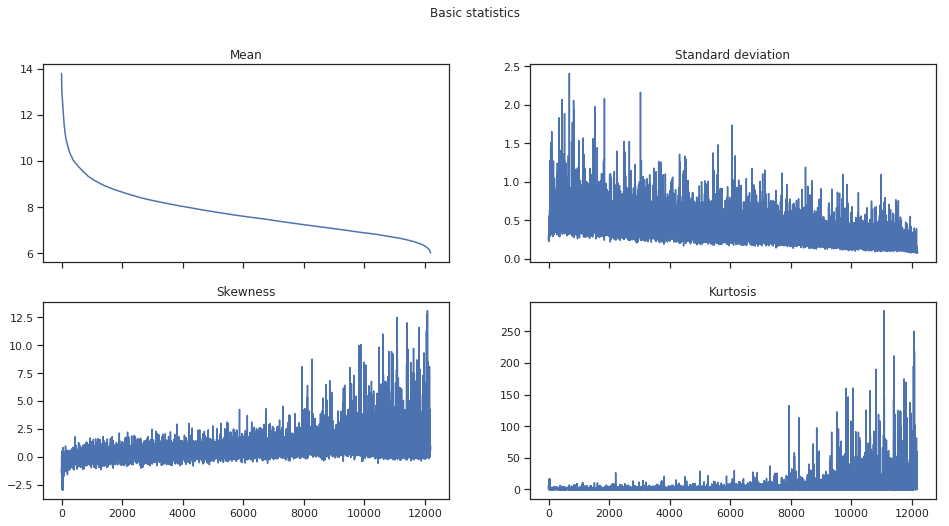
\includegraphics[width=\textwidth]{images/basic_stats.png}
\caption{Main statistical characteristics of the data}
\label{fig:stats}
\end{figure}

On the figure \ref{fig:stats} we can see that the data is not standardized. The variables are sorted decreasingly by means varying from $6.01$ to $13.79$. Also standard deviations vary from $0.07$ to $2.41$. Therefore, before applying any dimensionality reduction method we should standardize our data, e.g in PCA the variance explained by a variable hugely depends on its scale and could lack of standardization could lead to over or underestimation of its effect. Skewness and kurtosis evidence against our normality assumption.

They vary from $-2.99$ to $13.10$ and $-1.38$ to $282.88$ respectively. Especially, the kurtosis implies presence of outliers. In order to get more insight on the distribution of our variables in figure \ref{fig:hists_out} we plot the histogram and boxplots of genes with maximum skewness and kurtosis and in figure \ref{fig:hists_norm} we plot histograms and boxplots of randomly chosen genes from the data. 

\begin{figure}
\centering
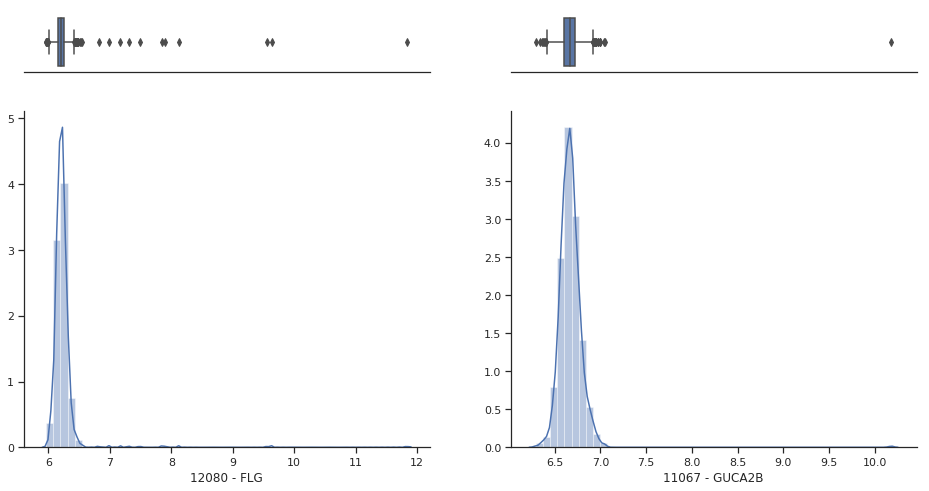
\includegraphics[width=\textwidth]{images/hists_ouliers.png}
\caption{Histograms of genes with maximum skewness and kurtosis}
\label{fig:hists_out}
\end{figure}

\begin{figure}
\centering
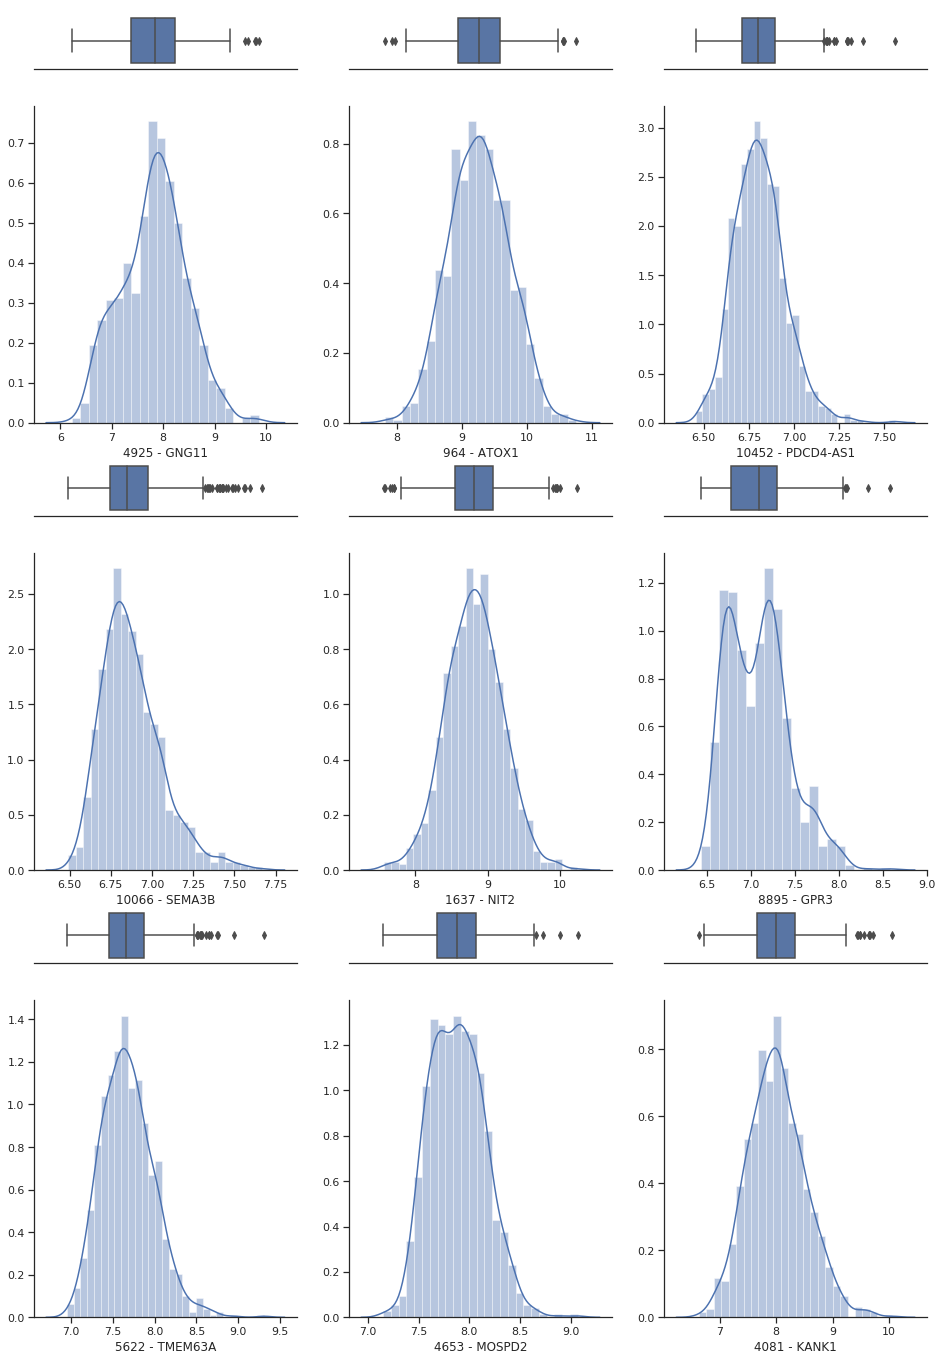
\includegraphics[width=\textwidth]{images/hists_normal.png}
\caption{Histograms of randomly chosen genes from the data}
\label{fig:hists_norm}
\end{figure}


By looking at the figure \ref{fig:hists_norm} we conclude that also the distribution are visibly skewed and even multimodal they do not indicate that further transformation is needed to able to use models assuming normality. However, we can clearly see form figure \ref{fig:hists_out} that high skewness or kurtosis can be caused by outlying values for this variable. In order to verify this we calculate the 95\% quantile for both skewness and kurtosis. They are equal to $2.15$ and $9.77$ respectively. It indicates that only very few genes have statistics indicating non normality. What is more, the number of genes with kurtosis or skewness above 95\% quantile is $710$ which is not significantly larger than the number of genes with high kurtosis only. This indicates that the extreme values of either of these statistics appear on the small subset of genes. In order to assess the influence of such genes we consider following data sets: data set consisting of genes only with values of skewness and kurtosis below the 95\% quantile ($D_1$), the complement of the previous data set ($D_2$), $50$ data sets extracted by randomly choosing $710$ variables from the original data ($D_{random}$). \textcolor{blue}{Wstawiać wykresy czy tylko score'y?} We split each of them to train and test parts and fit logistic regression with L1 penalty and regularization hyperparameter chosen using cross validation as described in section \ref{section:hypers}. We compare the scores on the test set (section \ref{section:scores}) to check how these genes with outlying values impact our prediction. For the random data sets we fit the model for each of them and take the mean scores. The results are presented in the table below: 
\begin{table}[H]
\centering
    \begin{tabular}[t]{c c c c c}
    \toprule
    & ROC AUC & Precision & Recall & F1\\
    \midrule
    $D_1$ & $0.832$ & $0.667$ &	$0.660$ & $0.663$ \\
    $D_2$ & $0.727$ & $0.678$ & $0.570$ & $0.619$ \\
    $D_{random}$ & $0.777$ & $0.687$ & $0.590$ & $0.633$ \\
    \bottomrule
\end{tabular}
    \caption{Scores of logistic regression with subsets of variables}
    \label{tab:scores-trunc}
\end{table}

From this table we can clearly see that the genes in $D_2$ do not have big predictive power. The mean scores from $D_{random}$ are higher for every considered metric. It is also worth noting that randomly chosen variables bring less information for prediction than all the genes in $D_1$, especially in terms of recall. The next step is checking how these genes with extreme values impact prediction.

\begin{itemize}
    \item Description
    \item Basic statistics
    \item Normalization
    \item Heatmap
\end{itemize}

\section{Results}


\section{Applications in medicine}

\begin{itemize}
    \item What is acceptable in medicine
    \item Not liking black box models
    \item Linear vs nonlinear
    \item Feature extraction vs feature selection
    \item comparison with other papers
    \item pathway enrichment
\end{itemize}

\section{Conclusion}

\bibliography{biblio}
\bibliographystyle{plain}
%\bibliographystyle{apalike}


\end{document}
